

\begin{figure}[htbp]
\centerline{\includegraphics[width=\linewidth]{"./fig 1.png"}}
\caption{fig 1.}
\label{fig}
\end{figure}


\begin{figure}[htbp]
\centerline{\includegraphics[width=\linewidth]{"./Number of characters, distribution in corpus.png"}}
\caption{Number of characters, distribution in corpus.}
\label{fig}
\end{figure}


\begin{figure}[htbp]
\centerline{\includegraphics[width=\linewidth]{"./Number of lines, distribution in corpus.png"}}
\caption{Number of lines, distribution in corpus.}
\label{fig}
\end{figure}


\begin{figure}[htbp]
\centerline{\includegraphics[width=\linewidth]{"./Number of tokens, distribution in corpus.png"}}
\caption{Number of tokens, distribution in corpus.}
\label{fig}
\end{figure}


\begin{figure}[htbp]
\centerline{\includegraphics[width=\linewidth]{"./Number of sentences in summary.png"}}
\caption{Number of sentences in summary.}
\label{fig}
\end{figure}


\begin{figure}[htbp]
\centerline{\includegraphics[width=\linewidth]{"./Number of sentences in <think> section.png"}}
\caption{Number of sentences in <think> section.}
\label{fig}
\end{figure}


\begin{figure}[htbp]
\centerline{\includegraphics[width=\linewidth]{"./Number of words in summary.png"}}
\caption{Number of words in summary.}
\label{fig}
\end{figure}


\begin{figure}[htbp]
\centerline{\includegraphics[width=\linewidth]{"./Number of words in <think> section.png"}}
\caption{Number of words in <think> section.}
\label{fig}
\end{figure}


\begin{figure}[htbp]
\centerline{\includegraphics[width=\linewidth]{"./Comparing number of characters in the corpus vs the reconstructed models.png"}}
\caption{Comparing number of characters in the corpus vs the reconstructed models.}
\label{fig}
\end{figure}


\begin{figure}[htbp]
\centerline{\includegraphics[width=\linewidth]{"./Comparing number of lines in the corpus vs the reconstructed models.png"}}
\caption{Comparing number of lines in the corpus vs the reconstructed models.}
\label{fig}
\end{figure}


\begin{figure}[htbp]
\centerline{\includegraphics[width=\linewidth]{"./Comparing number of tokens in the corpus vs the reconstructed models.png"}}
\caption{Comparing number of tokens in the corpus vs the reconstructed models.}
\label{fig}
\end{figure}


\begin{figure}[htbp]
\centerline{\includegraphics[width=\linewidth]{"./correlation between size of original and reconstructed model.png"}}
\caption{correlation between size of original and reconstructed model.}
\label{fig}
\end{figure}


\begin{figure}[htbp]
\centerline{\includegraphics[width=\linewidth]{"./correlation between size of model and LLM-generated summary.png"}}
\caption{correlation between size of model and LLM-generated summary.}
\label{fig}
\end{figure}


\begin{figure}[htbp]
\centerline{\includegraphics[width=\linewidth]{"./Comparing number of comments in the corpus vs the reconstructed models.png"}}
\caption{Comparing number of comments in the corpus vs the reconstructed models.}
\label{fig}
\end{figure}


\begin{figure}[htbp]
\centerline{\includegraphics[width=\linewidth]{"./Comparing total number of words in the comments in the corpus vs the reconstructed models.png"}}
\caption{Comparing total number of words in the comments in the corpus vs the reconstructed models.}
\label{fig}
\end{figure}


\begin{figure}[htbp]
\centerline{\includegraphics[width=\linewidth]{"./Comparing number of signatures in the corpus vs the reconstructed models.png"}}
\caption{Comparing number of signatures in the corpus vs the reconstructed models.}
\label{fig}
\end{figure}


\begin{figure}[htbp]
\centerline{\includegraphics[width=\linewidth]{"./Comparing size of the signature bodies in the corpus vs the reconstructed models.png"}}
\caption{Comparing size of the signature bodies in the corpus vs the reconstructed models.}
\label{fig}
\end{figure}


\begin{figure}[htbp]
\centerline{\includegraphics[width=\linewidth]{"./Correlation between number of signatures in the original and reconstructed models.png"}}
\caption{Correlation between number of signatures in the original and reconstructed models.}
\label{fig}
\end{figure}


\begin{figure}[htbp]
\centerline{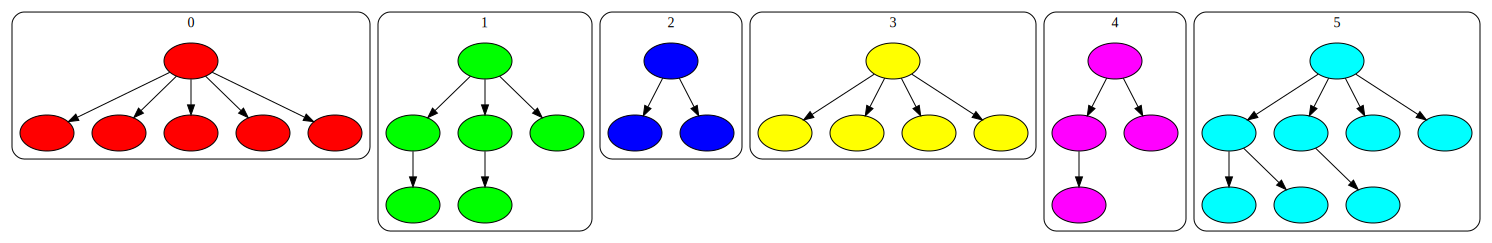
\includegraphics[width=\linewidth]{"./distribution of inheritance hierarchies (original).png"}}
\caption{distribution of inheritance hierarchies (original).}
\label{fig}
\end{figure}


\begin{figure}[htbp]
\centerline{\includegraphics[width=\linewidth]{"./distribution of inheritance hierarchies (reconstructed).png"}}
\caption{distribution of inheritance hierarchies (reconstructed).}
\label{fig}
\end{figure}


\begin{figure}[htbp]
\centerline{\includegraphics[width=\linewidth]{"./Distribution of ratings from manual analysis.png"}}
\caption{Distribution of ratings from manual analysis.}
\label{fig}
\end{figure}


\begin{figure}[htbp]
\centerline{\includegraphics[width=\linewidth]{"./Comparing number of asserts in the corpus vs the reconstructed models.png"}}
\caption{Comparing number of asserts in the corpus vs the reconstructed models.}
\label{fig}
\end{figure}


\begin{figure}[htbp]
\centerline{\includegraphics[width=\linewidth]{"./Correlation between number of asserts in the original and reconstructed models.png"}}
\caption{Correlation between number of asserts in the original and reconstructed models.}
\label{fig}
\end{figure}


\begin{figure}[htbp]
\centerline{\includegraphics[width=\linewidth]{"./Comparing number of facts in the corpus vs the reconstructed models.png"}}
\caption{Comparing number of facts in the corpus vs the reconstructed models.}
\label{fig}
\end{figure}


\begin{figure}[htbp]
\centerline{\includegraphics[width=\linewidth]{"./Correlation between number of facts in the original and reconstructed models.png"}}
\caption{Correlation between number of facts in the original and reconstructed models.}
\label{fig}
\end{figure}


\begin{figure}[htbp]
\centerline{\includegraphics[width=\linewidth]{"./Comparing number of funs in the corpus vs the reconstructed models.png"}}
\caption{Comparing number of funs in the corpus vs the reconstructed models.}
\label{fig}
\end{figure}


\begin{figure}[htbp]
\centerline{\includegraphics[width=\linewidth]{"./Correlation between number of funs in the original and reconstructed models.png"}}
\caption{Correlation between number of funs in the original and reconstructed models.}
\label{fig}
\end{figure}


\begin{figure}[htbp]
\centerline{\includegraphics[width=\linewidth]{"./Comparing number of preds in the corpus vs the reconstructed models.png"}}
\caption{Comparing number of preds in the corpus vs the reconstructed models.}
\label{fig}
\end{figure}


\begin{figure}[htbp]
\centerline{\includegraphics[width=\linewidth]{"./Correlation between number of preds in the original and reconstructed models.png"}}
\caption{Correlation between number of preds in the original and reconstructed models.}
\label{fig}
\end{figure}
